This chapter creates an understanding of the available data, how it is analysed and prepared before including it in deep learning models. Additionally, the program Navigate Pain and programs used to development of the deep learning models are described. Furthermore, the implementation of the deep learning model is presented consisting of hardware, software and architecture of used neural network.

\section{Data description}
Data used in this project were collected beforehand from an on-going FOXH trial which is conducted in collaboration with Danish and Australian universities. The data consists of pain maps which were drawn by individuals with PFP syndrome through the use of an application, Navigate Pain, in a clinical setting. Navigate pain is further described in section \ref{sec:nav}. The pain maps are both from individuals with uni- and bilateral PFP. An example of a pain drawing with bilateral pain is shown in figure \ref{fig:kneepainmap}.

\begin{figure} [H]
\centering
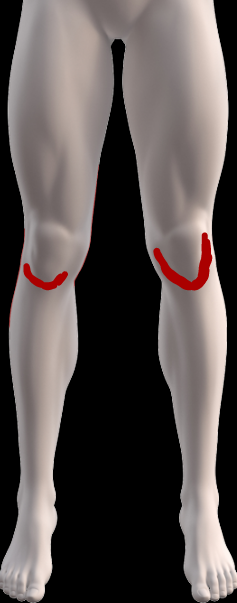
\includegraphics[width=0.2\textwidth]{figures/kneepainmap}
\caption{An example of a pain drawing from individual with PFP syndrome. The red markings indicate the area of pain perceived by the individuals. In this case the PFP is bilateral (on both knees).}
\label{fig:kneepainmap}
\end{figure}

\noindent
In addition to the pain maps a corresponding dataset was available. This contained information regarding the individuals in terms of i.a. age, gender, pain duration, and intensity and the most prominent knee for pain. However, not all of the information was present for all individuals.
Before using the data in the deep learning models, a manual data handling was necessary. This incorporated matching the given pain maps and associated ID regarding the individuals. Furthermore, specific information like gender, pain duration, and intensity were collected.\newline
\noindent
To create more pain maps a split body approach was used, which contained splitting pain maps in two legs, whereafter the pain on left knees was mirrored and only visualized on the right knee. This resulted in 333 pain maps with associated pain duration, and 319 pain maps associated with pain intensity. 



\subsection{Software application: Navigate Pain} \label{sec:nav}
Navigate Pain is a software application that is used to visualise the location, shape and spatial distribution of pain from individuals to healthcare personnel. The application permits individuals to draw their pain into a body outline. Navigate Pain android was developed at Aalborg University, and a commercial web application is available at Aglance Solutions (Denmark).\citep{Solutions2015}
\autoref{fig:Navigatepain} illustrates the process using the application.

\begin{figure} [H]
\centering
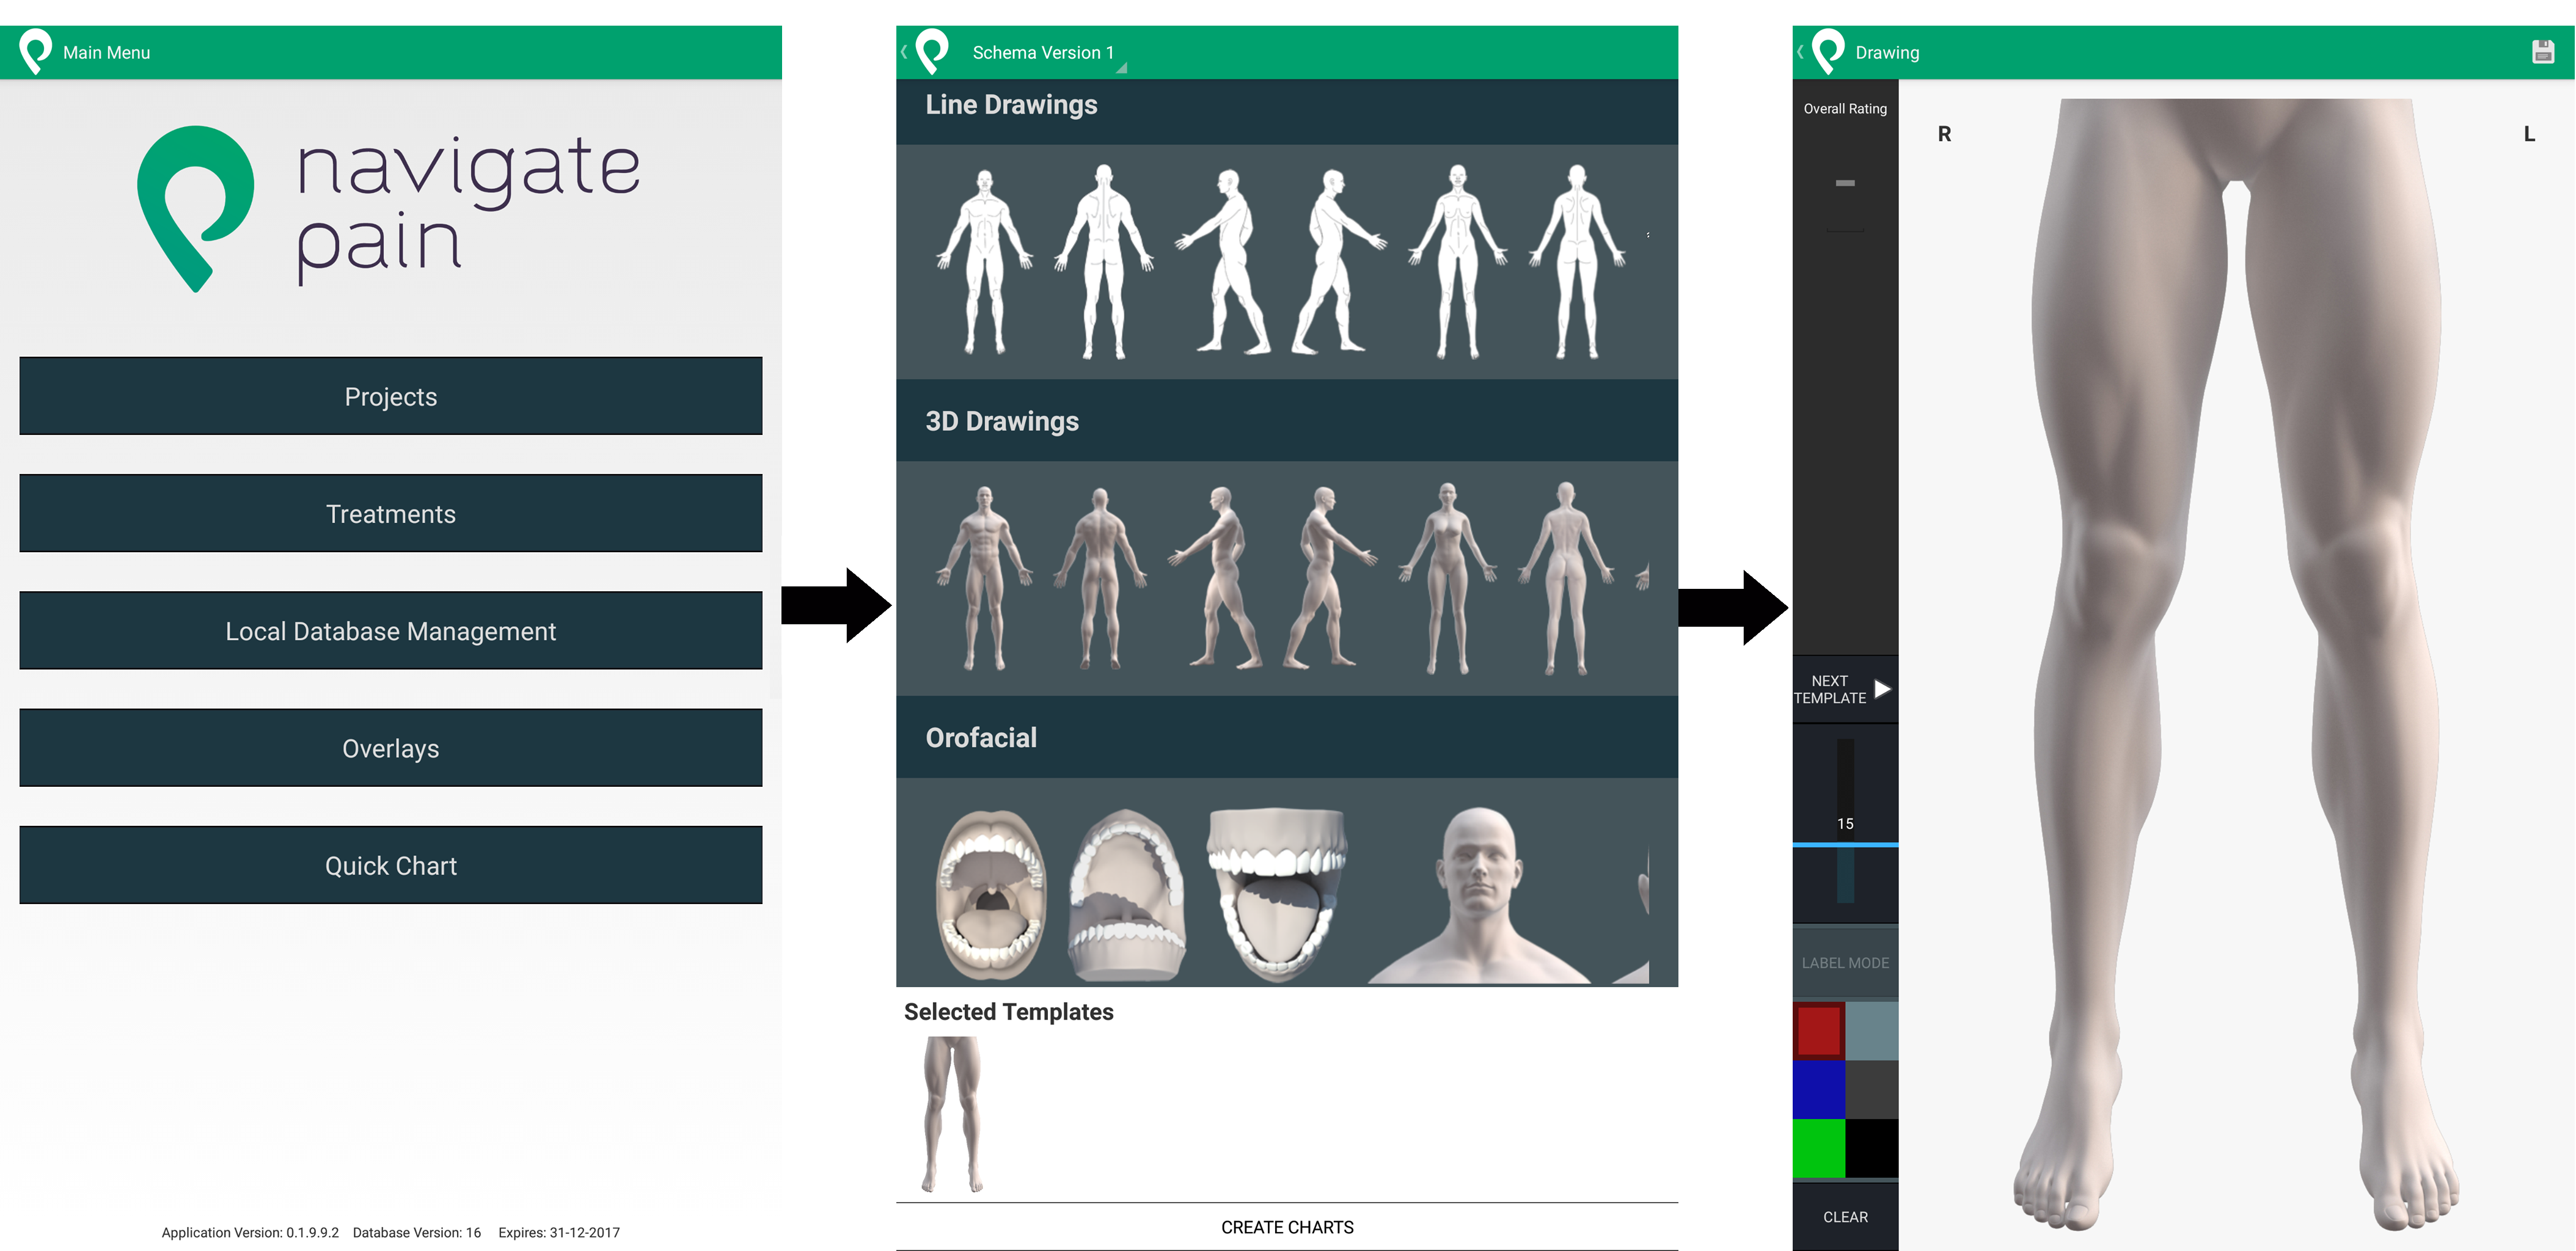
\includegraphics[width=1\textwidth]{figures/Navigatepain}
\caption{The process for making a pain map with Navigate Pain. (a) shows the main screen, (b) categories of body outlines and (c) body outline for lower extremities.}
\label{fig:Navigatepain}
\end{figure}

\noindent
In figure \ref{fig:Navigatepain}(a) is the main screen. By clicking on "Projects", a folder with individuals is created. For each individual, information like name, age, height is saved. Before the individual can draw their pain areas, the body outline has to be chosen, which is illustrated in figure \ref{fig:Navigatepain}(b). The body outlines are divided into five categories: Line Drawings, 3D Drawings, Orofacial, Special Zooms and Knee Pain. In the bottom the seleceted templates are shown. When clicking on "create charts" the screen in figure \ref{fig:Navigatepain}(c) is shown. Here it is possible to draw the pain areas with different colors and line thickness, which can be seen in the left side of the screen. Afterwards, the pain map can be saved.


\subsection{Data representations} \label{sec:representation}
It is presumed that different representations of the pain maps affect the performance accuracy of a deep learning models, hence different data representations were created.
A study by \citeauthor{Boudreau2017} \citep{Boudreau2017} found a partial correlation between a prolonged pain duration and the size of the pain area. It was shown that the pain area increased for individuals that had a pain duration for longer than five years. Likewise, pain intensity had a correlation with the size of pain area for individuals with a pain duration for more than five years. Furthermore, the shape of the pain developed from a U-shape to an O-shape for individuals with a pain duration above five years.\citep{Boudreau2017} \newline
\noindent
It is unknown whether the morphology or location of the pain influence either pain duration or intensity to which two data representations reflecting morphology or locations of the pain are created.
A combination of the two data representations is created to achieve a third data representation which both include the morphology of the pain and the location, which is defined using the knee regions. The three data representations are referred to as morphology-, location- and combined-representation.
\noindent
Furthermore, gender may be considered as an important parameter to use as an input, because of the difference in how females and males report their pain. Additionally, there is an imbalance in prevalence.

\begin{figure} [H]
\centering
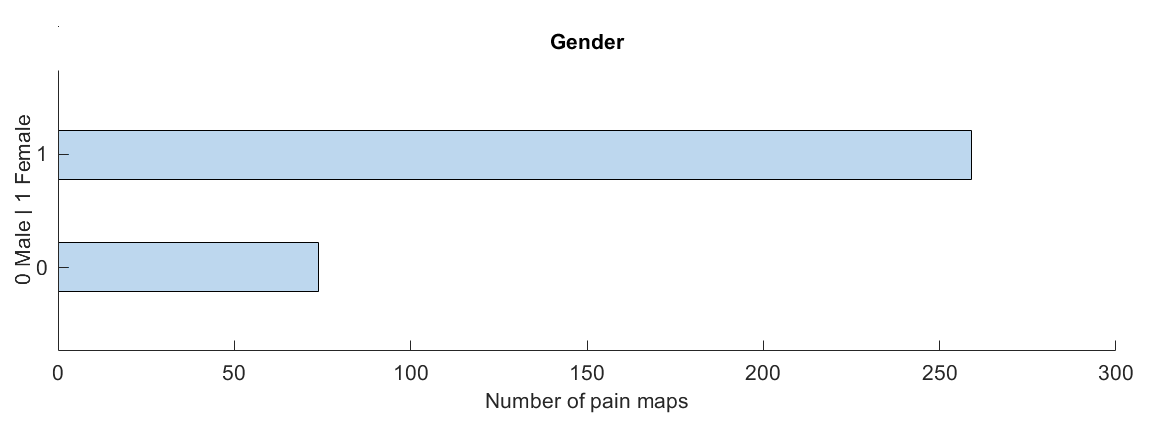
\includegraphics[width=1\textwidth]{figures/histoGender}
\caption{Histogram of the distribution of gender.}
\label{fig:histogender}
\end{figure}

\noindent
According to the given data the distribution is higher for females than males. The females constitute 259 of the 333 individuals, and males constituted 74 individuals.  \newline

\section{Pre-analysis}
The pain maps and associated pain duration as well as pain intensity are analysed to get an overview of the data. The data is analysed in MatLab, where the distribution of the outputs, pain duration and intensity, are investigated whereafter intervals used for classification in the deep learning models are decided. Furthermore, different threshold values are analysed according to five pain maps to select the threshold which should define when a pain region is considered active.
Simple linear regressions are made to investigate whether pain duration or intensity have a linear relation to the size of pain.


\subsection{Classification of data}
The deep learning models should classify the input, pain maps and gender, in different intervals in relation to pain duration or intensity intervals. To help define the class intervals of both pain duration and intensity, histograms are created.

\noindent
A histogram of the pain duration associated with the pain maps is illustrated in figure \ref{fig:histoduration}.

\begin{figure} [H]
\centering
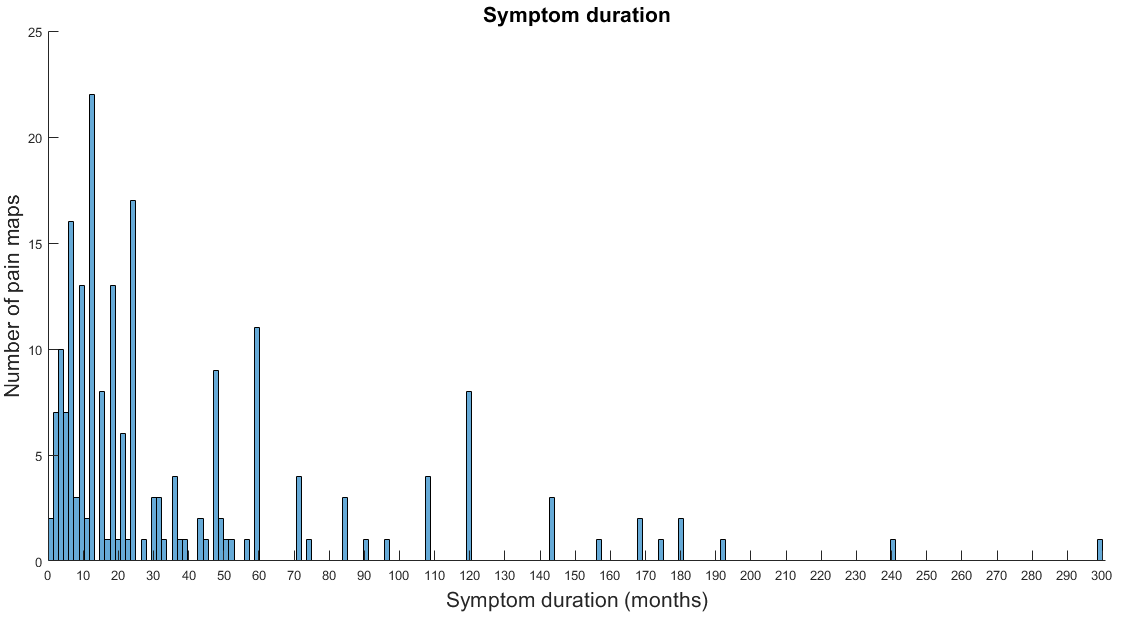
\includegraphics[width=1\textwidth]{figures/histogramDuration}
\caption{A histogram of the pain duration according to the number of pain maps.}
\label{fig:histoduration}
\end{figure}

\noindent
The pain duration is divided into some classes which the models should classify in according to. To test the models the data firstly are divided into two extremes, since it is assumed that if the models predict badly with the extremes, the models will not predict better with multiple classifications of pain duration. 
By considering the amount of data and the distribution shown in the histogram class intervals were chosen to be 0 to 12 months (n=144), and 36 to 300 months (n=122). \newline

\noindent
In the associated data to the pain map the individuals have stated their pain intensity as the worst pain in the last 24 hours and the last seven days.
It is not assumably that the individuals have performed any PFP provoked activity in the last 24 hours before drawing their pain, therefore it is chosen to use the worst pain intensity in the last seven days to get a more average value for the worst pain intensity.
To illustrate the distribution of the individuals’ worst pain intensity in the last seven days a histogram is created which can be seen in figure \ref{fig:histopain}.

\begin{figure} [H]
\centering
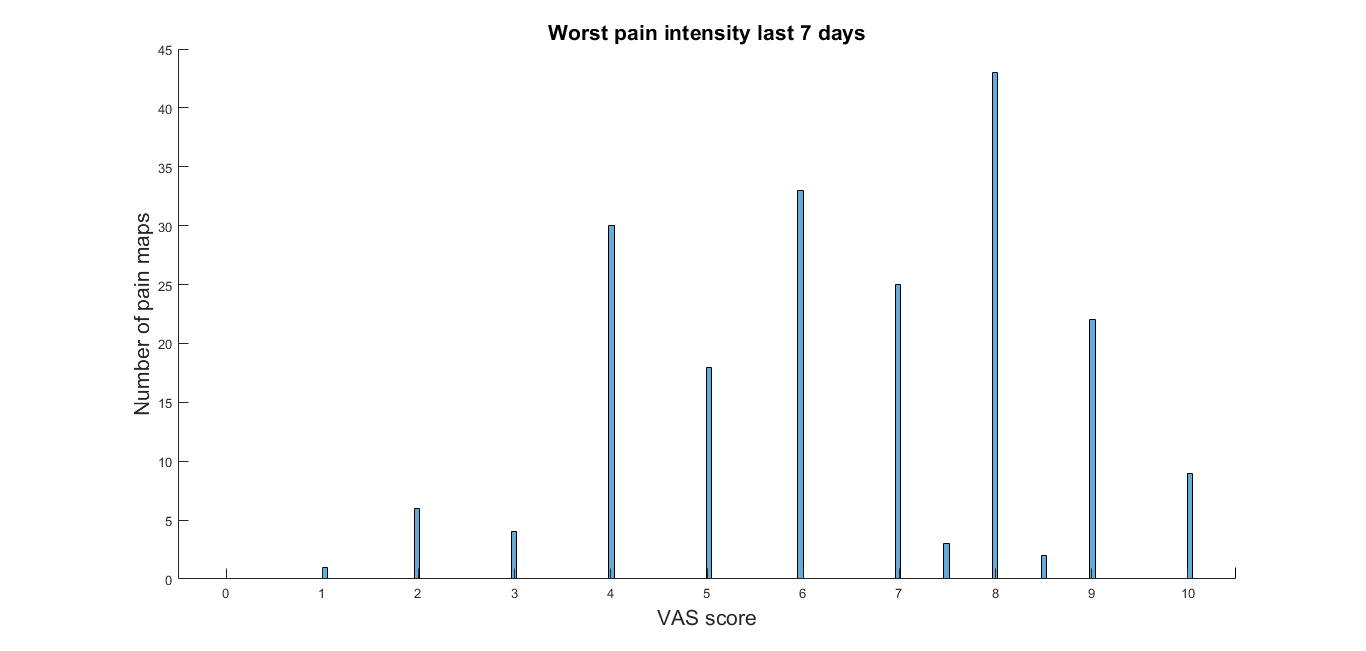
\includegraphics[width=1\textwidth]{figures/histrogramPain}
\caption{A histogram of the worst pain intensity in the last seven days according to the number of pain maps. }
\label{fig:histopain}
\end{figure}

\noindent
Likewise to the pain duration classification, the worst pain intensity is divided into the extremes, which are chosen to be intervals 1 to 4 (n=72) and 8 to 10 (n=124). The third classification constitute the interval between the extremes.


\subsection{Threshold selection}\label{sec:Selectthreshold}
In relation to the data representation that contains information about the location of the pain divided into knee regions, it is necessary to find a threshold that decides when a knee region contains enough pain pixels to be considered active. A threshold is required to increase the confidence of an active pain region by avoiding minimal contributions e.g. small pain areas in the associated regions. Simultaneously the threshold may not be too large so that potential pain regions will not be incorporated. The threshold to indicate active pain regions is decided based on an analysis, where threshold values of 5, 10 and 15\% are explored. A 0\% threshold is used as a reference. 
The analysis of the threshold is tested on five random pain maps to get a general impression of the data. To better distinguish the regions in figure \ref{fig:atlas} different colors are used as shown in figure \ref{fig:colorregion}


\begin{figure} [H]
\centering
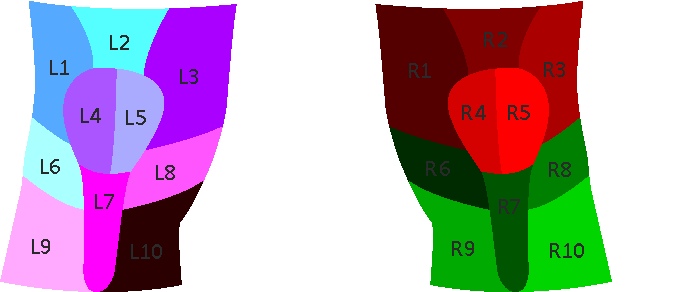
\includegraphics[width=0.25\textwidth]{figures/colorregion}
\caption{Knee regions colored to easier distinguish.}
\label{fig:colorregion}
\end{figure}

\noindent
An example of pain maps and related bar chart are illustrated in figure \ref{fig:threshold}. The pain maps are colored in the same colors as figure \ref{fig:colorregion} to indicate which regions are affected by pain according to \ref{fig:threshold}(a) no threshold, \ref{fig:threshold}(b) 5\% threshold, \ref{fig:threshold}(c) 10\% threshold and \ref{fig:threshold}(d) 15\% threshold. 
Figure \ref{fig:threshold}(e) shows a bar chart that indicates how many and which active regions there are according to the threshold values.

\begin{figure} [H]
\centering
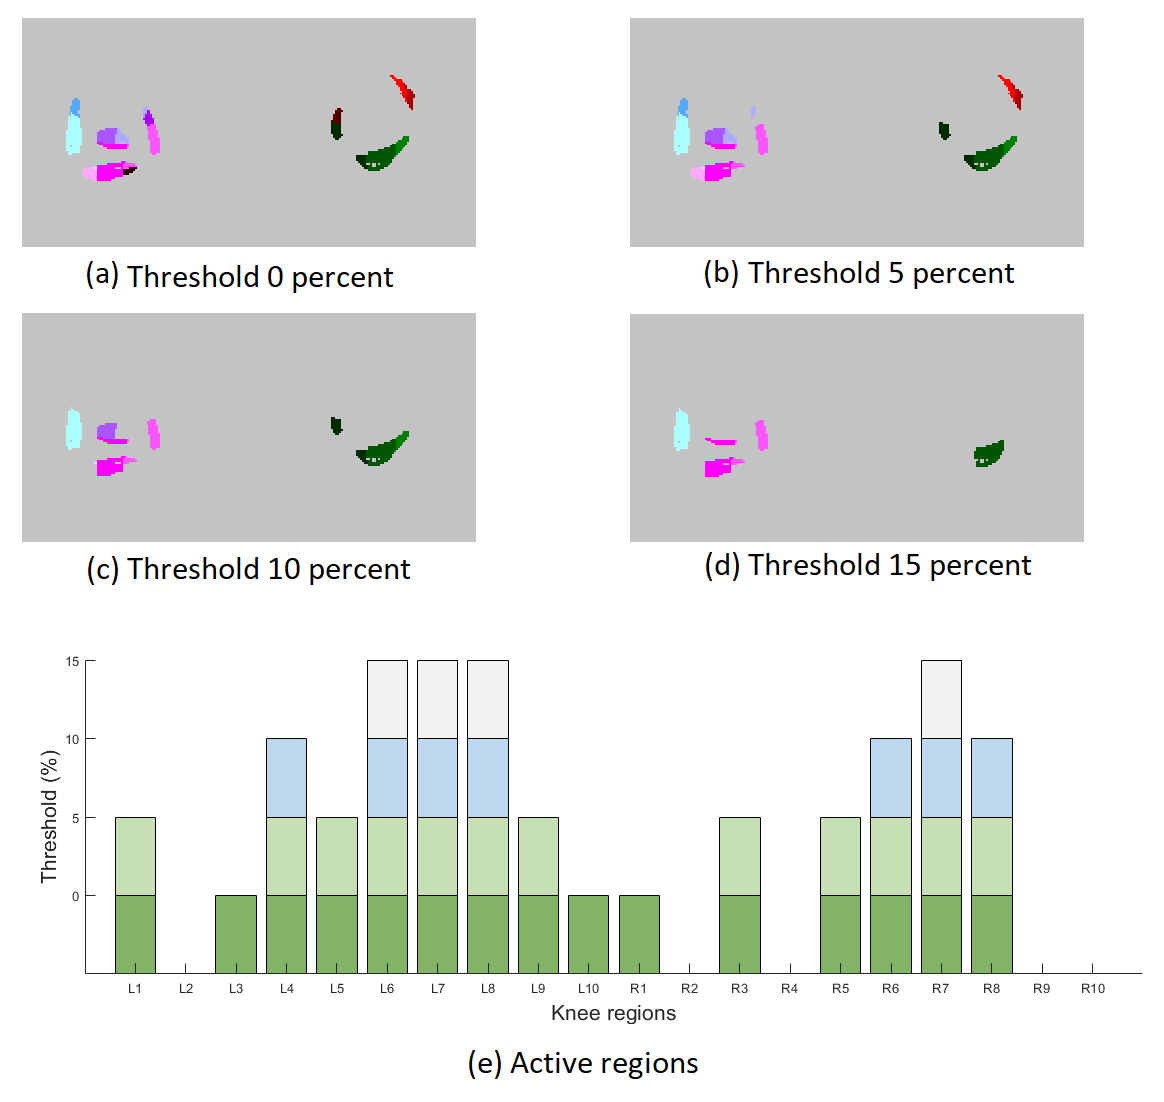
\includegraphics[width=0.95\textwidth]{figures/threshold4}
\caption{The active pain regions when the threshold is (a) 0\%, (b) 5\%, (c) 10\% and (d) 15\%. (e) is the bar chart that indicates how many and which regions that are considered active.}
\label{fig:threshold}
\end{figure}

\noindent
According to figure \ref{fig:threshold}(a) with no threshold, and (e) it is shown that the knee has nine active regions when no threshold is applied. In proportion to the active regions, pain regions R3 and R10 are very small and thereby the first regions to be discarded when the threshold is increased by 5\%, which is shown in figure (b).
By comparing figure (a) and (b) minor changes according to the missing regions can be seen, compared to figure (c) and (d) where greater areas disappears after increasing the threshold to 10 and 15\%.
\noindent
Based on analysis of the five pain maps and bar charts, in figure \ref{fig:threshold} and appendix \ref{app:thresholds}, a threshold on 5\% is chosen to avoid including minor pain areas, like region R10, as active pain regions, and to avoid discarding too many and large areas, like regions R4 and R5.


\subsection{Simple regression models}
To verify the assumption of complexity of pain maps, linear regressions on the data representations and output, pain duration or intensity, are created. 
Other features in the morphology- and location-representation are respectively the size of the pain (number of pain pixels) and the number of active regions. If these simple features have a linear correlation to the pain duration or intensity,  it may not be significant to investigate morphology and location as features in the deep learning models. \newline
\noindent
To investigate if pain size has a linear correlation to pain duration, a linear regression i created, which is shown in figure \ref{fig:durapixel}.
\newline

\begin{figure} [H]
\centering
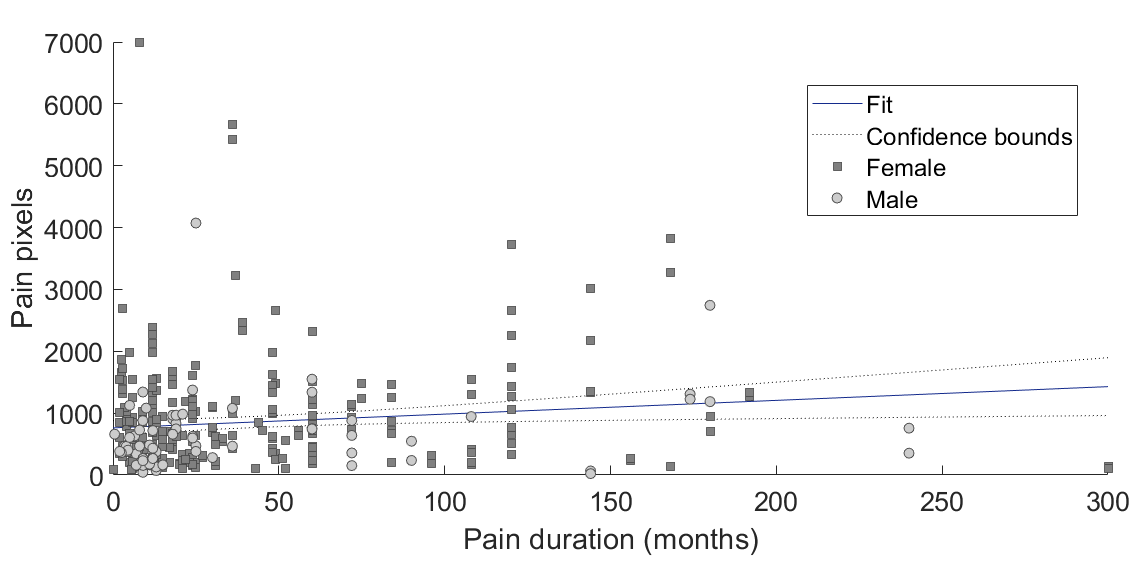
\includegraphics[width=1\textwidth]{figures/durapixel}
\caption{A linear regression of the the number of pain pixels and pain duration.}
\label{fig:durapixel}
\end{figure}

\noindent
As a result of the linear regression model is $R^2=0.046$, which indicates that there is no linear correlation between the number of pain pixels and pain duration.\newline
\noindent
A linear regression model of the number of pain pixels and pain intensity is made, which is shown in figure \ref{fig:painRegression}. \newline

\begin{figure} [H]
\centering
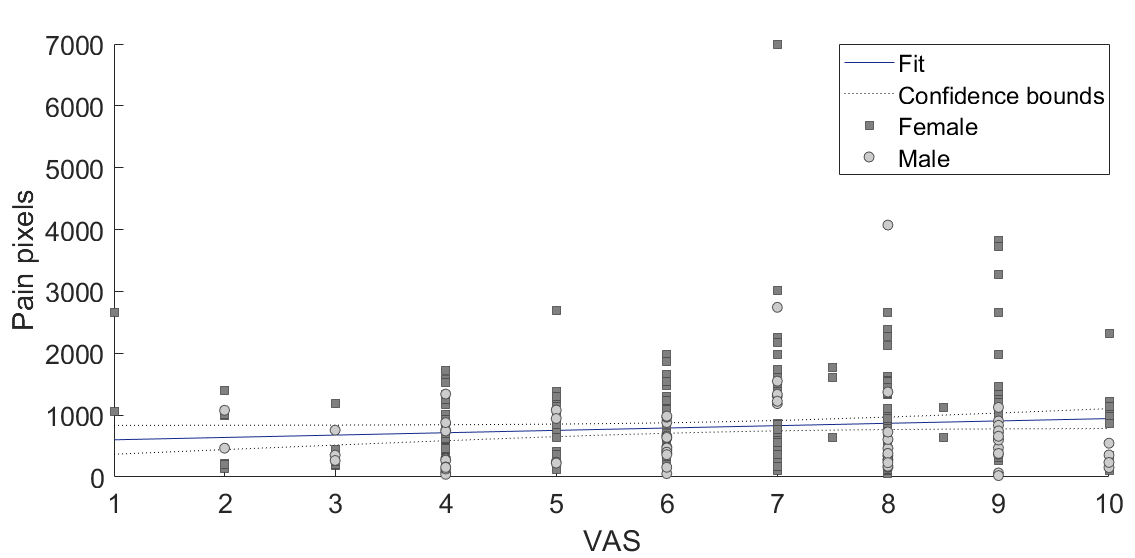
\includegraphics[width=1\textwidth]{figures/vaspixel}
\caption{A linear regression of the number of pain pixels and pain intensity stated in VAS.}
\label{fig:painRegression}
\end{figure}

\noindent
The result in this linear regression is $R^2=0.0117$, which indicates that there is no any linear correlation to be found between the number of pain pixels and pain intensity.\newline

\noindent
These linear regression models are not very suitable when trying to find a correlation between the number of pain pixels and pain duration or intensity. However, they can be compared to the performance of the deep learning models.


\noindent
A linear regression between the number of active pain regions with a threshold on 5\% and pain duration is shown in figure \ref{fig:regDuration}. \newline

\begin{figure} [H]
\centering
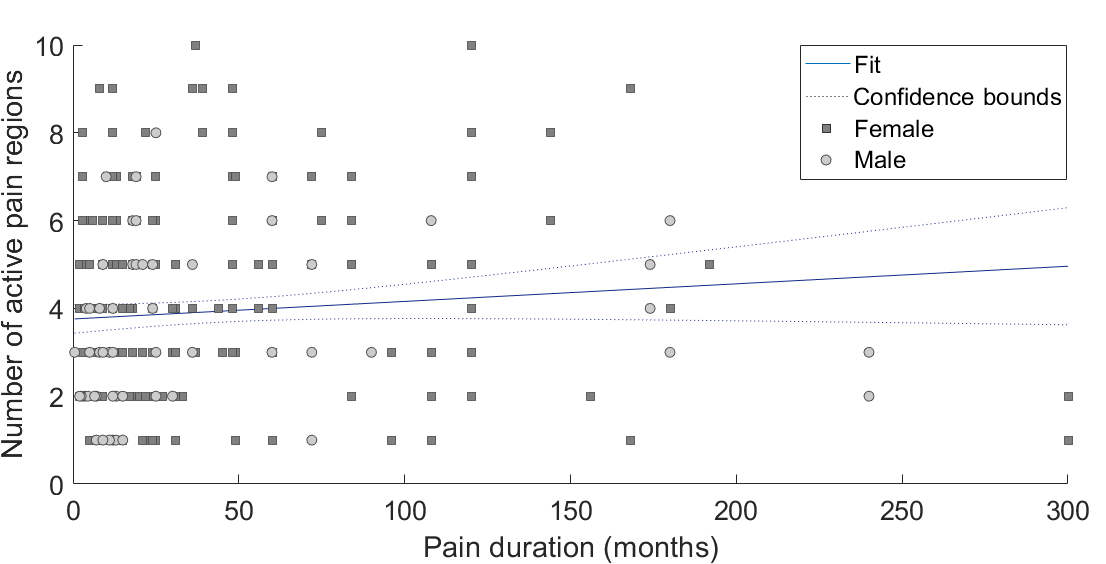
\includegraphics[width=1\textwidth]{figures/duraregion}
\caption{A linear regression of the number of active pain regions and pain duration.}
\label{fig:regDuration}
\end{figure}

\noindent
The result in this linear regression between the number of active pain regions and pain duration is $R^2=0.0357$, which indicates that there is no any linear correlation to be found.\newline
Thereto, a linear correlation between the number of active pain regions and pain intensity is shown in figure \ref{fig:regPain}.

\begin{figure} [H]
\centering
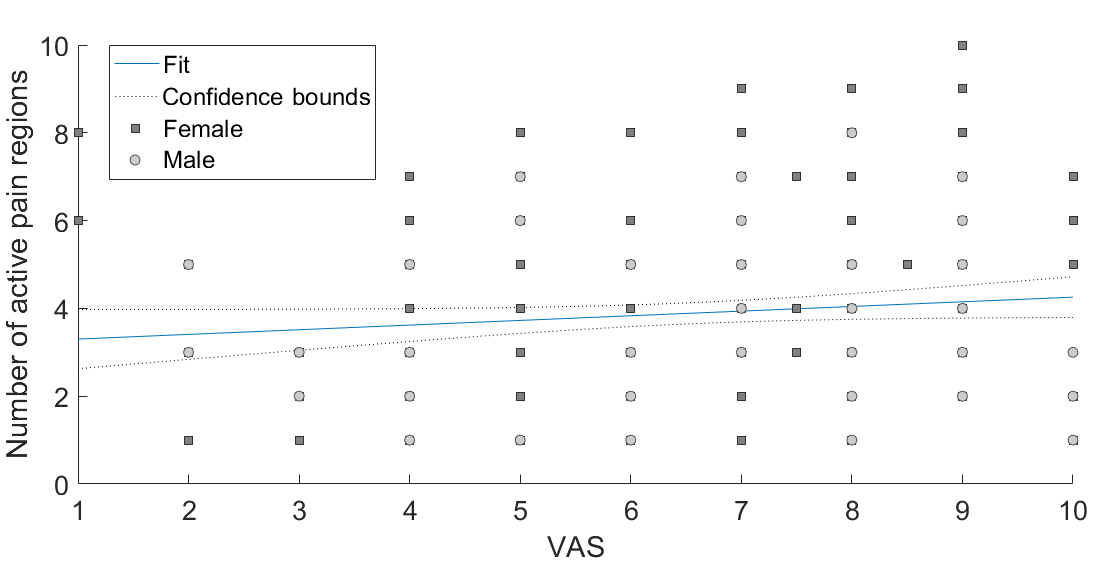
\includegraphics[width=1\textwidth]{figures/vasregion}
\caption{A linear regression of the number active pain regions and pain intensity.}
\label{fig:regPain}
\end{figure}

\noindent
The result of the linear regression between the number of active pain regions and pain intensity is $R^2=0.00833$, which once again indicates nonlinearity. 

\noindent
Based on the four linear regression models, it is assumed that a single feature, number of pain pixels or number of active pain regions with a 5\% threshold, may not have a simple correlation with the outputs, pain duration or intensity. Hence a deep learning model may find patterns in the pain maps in relation to either pain duration or intensity.



\section{Pre-processing} \label{sec:prepros}
The data is pre-processed in MatLab to prepare the three different data representations. The three data representations are morphology-, location-, and combined-representation, which are described in section \ref{sec:representation}. Common for the data representation is that the pain maps are imported as image-matrices whereafter the matrices are resized (pixelsize: $252 \times 118 = 29,736$), since the given pain maps were collected at different resolutions (screen sizes). Furthermore, the matrices are cropped to sort out unnecessary data.
Before the data is used as an input in the deep learning models, each matrix which represent an image, is converted into a vector whereafter they are assembled in one matrix for each data representation. To get additional information associated with the pain maps, gender is added by including a column vector to the three matrices.
In addition to the input, a classification label is added. The label, which is either pain duration or intensity, is added as a column vector.
The following sections describe the pre-processing of the individual data representations.

\subsection{Morphology-representation} \label{sec:Morph}
The first representation of data is a binary matrix of the original pain maps.
Firstly, the image of the original pain map is gray-scaled to get a one-dimensional matrix instead of a three-dimensional RGB-matrix. This matrix is then converted into a matrix consisting of zeroes and ones, where the pain pixels are defined with a value of one. An original pain map and a pain map consisting of a binary matrix is shown in figure \ref{fig:cropbin7}.

\begin{figure} [H]
\centering
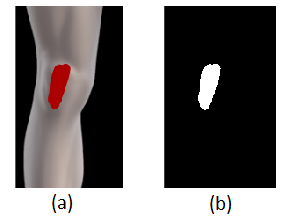
\includegraphics[width=0.5\textwidth]{figures/cropbin7}
\caption{(a) Original pain map and (b) image consisting of a binary matrix where white color represents the pain pixels.}
\label{fig:cropbin7}
\end{figure}

\noindent
An illustration of this morphology-representation is created to convey how the data is assembled and transferred to the model. The illustration is shown in figure \ref{fig:binmatrix}, where a matrix containing image-vectors for all the pain maps and appurtenant gender and either pain duration or intensity.

\begin{figure} [H]
\centering
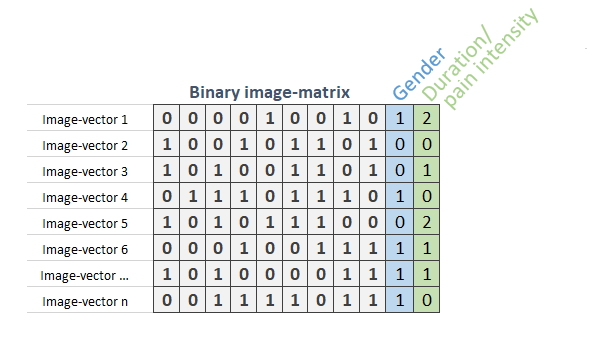
\includegraphics[width=0.8\textwidth]{figures/binaryimagematrix}
\caption{An illustration of the matrix of the morphology-representation. The matrix consists of image-vectors for each individuals where the two last columns indicate the corresponding gender (blue column vector) and either pain duration or intensity (green column vector). The image-vectors have a length equal to the number of pixels in the pain maps.}
\label{fig:binmatrix}
\end{figure}


\subsection{Location-representation} \label{sec:Regions}
The second representation of the data is a matrix consisting of vectors with 10 values which indicate location of pain in relation to the knee regions.
Figure \ref{fig:atlas} is cropped, and converted into a matrix consisting of 10 values, which represent each knee region on the right knee. This matrix is superimposed on the binary image of the pain map, which results in a matrix with pain pixels represented in each knee region. 
An illustration of the knee regions and an example of a pain map with the pain divided into regions are shown in figure \ref{fig:binregions}.

\begin{figure} [H]
\centering
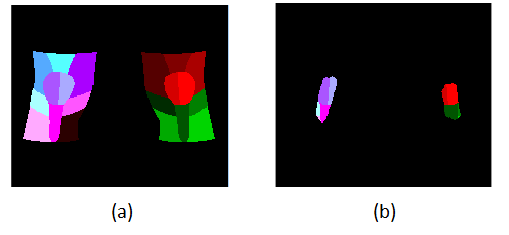
\includegraphics[width=0.6\textwidth]{figures/binregions}
\caption{(a) Knee regions and (b) an example of a pain map with pain in the specific regions.}
\label{fig:binregions}
\end{figure}

\noindent
After superimposing the two matrices, knee regions and pain pixels, the number of pain pixels in each active pain region is found. This number is compared to the total number of pixels that are in each knee region, so knee regions with less than 5\% pain are excluded. The threshold on 5\% is chosen based on the analysis in section \ref{sec:Selectthreshold}. As a result a vector with 10 values is created with zeros and ones, where one represent an active pain region. Location-representation is imported in the deep learning models the same way as the morphology-representation, which is illustrated in figure \ref{fig:binmatrix}. The only difference is that the length of the image-vectors respond to the 10 regions, and therefore there are only 10 values for each pain map.


\subsection{Combined-representation} \label{sec:combined}
The third representation of the data is a matrix consisting the morphology of pain divided into the knee regions.
\noindent
In this representation the superimposed matrix from the location-representation is used. Additionally one-hot encoding is used to divide the pain into different knee regions. One-hot encoding is a way to separate categorical data into binary data \citep{Harris2012}. This means that the 10 values do not have a correlation when analysed in the deep learning model. After one-hot encoding, the superimposed matrix consists of 10 layers where each layer represents a knee region, which is illustrated in figure \ref{fig:onehot}(a), and afterwards converted to image-vector with gender and the output as illustrated in figure \ref{fig:onehot}(b).

\begin{figure} [H]
\centering
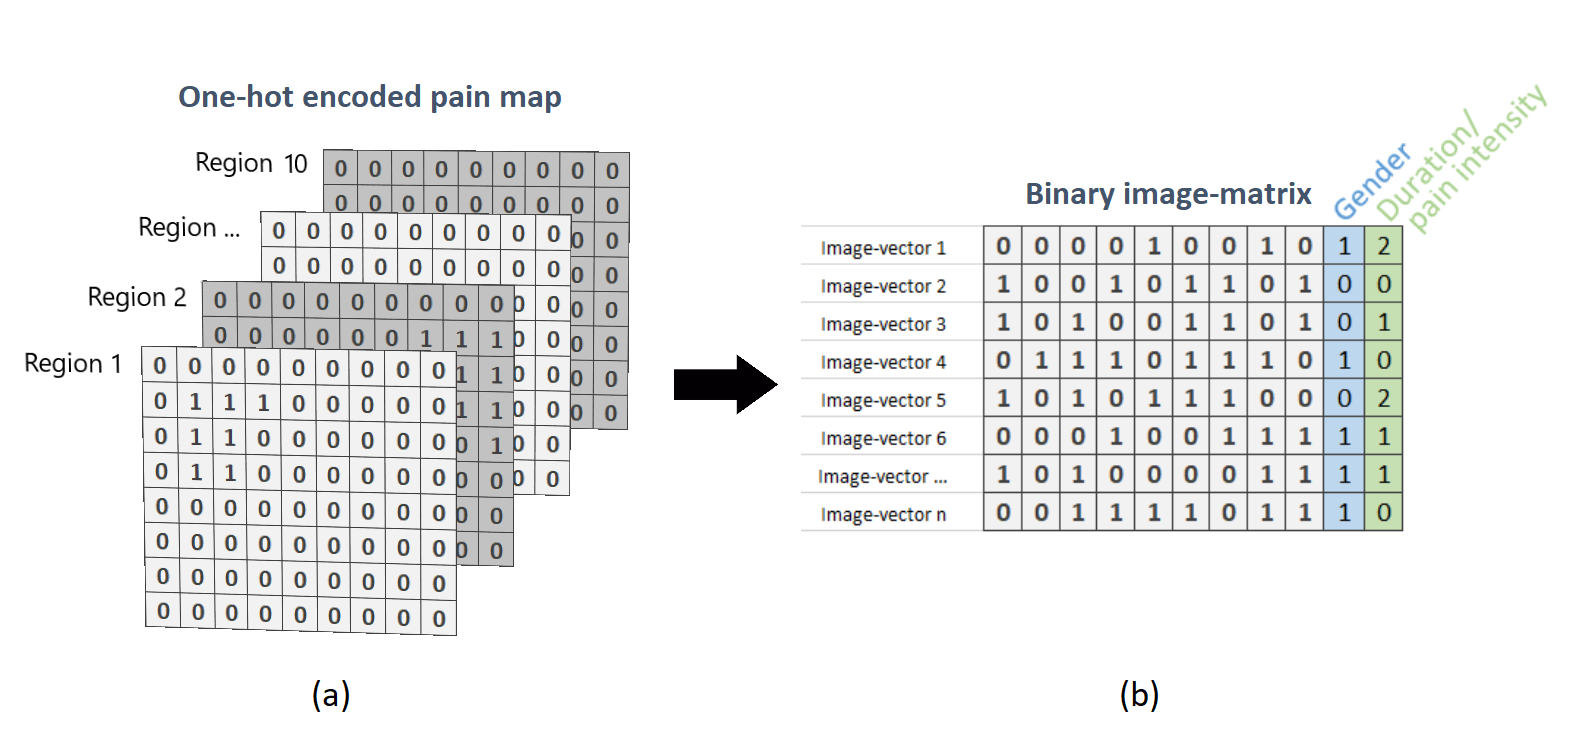
\includegraphics[width=1\textwidth]{figures/onehotmatrix}
\caption{(a) An illustration of a one-hot encoded pain map and (b) shows the image-vectors in one assembled matrix with gender and either pain duration or intensity.}
\label{fig:onehot}
\end{figure}
